% $Id: template.tex 11 2007-04-03 22:25:53Z jpeltier $

%\documentclass{vgtc}                          % final (conference style)
%\documentclass[review]{vgtc}                 % review
%\documentclass[widereview]{vgtc}             % wide-spaced review
%\documentclass[preprint]{vgtc}               % preprint
\documentclass[electronic]{vgtc}             % electronic version

%% Uncomment one of the lines above depending on where your paper is
%% in the conference process. ``review'' and ``widereview'' are for review
%% submission, ``preprint'' is for pre-publication, and the final version
%% doesn't use a specific qualifier. Further, ``electronic'' includes
%% hyperreferences for more convenient online viewing.

%% Please use one of the ``review'' options in combination with the
%% assigned online id (see below) ONLY if your paper uses a double blind
%% review process. Some conferences, like IEEE Vis and InfoVis, have NOT
%% in the past.

%% Figures should be in CMYK or Grey scale format, otherwise, colour 
%% shifting may occur during the printing process.

%% These few lines make a distinction between latex and pdflatex calls and they
%% bring in essential packages for graphics and font handling.
%% Note that due to the \DeclareGraphicsExtensions{} call it is no longer necessary
%% to provide the the path and extension of a graphics file:
%% \includegraphics{diamondrule} is completely sufficient.
%%
\ifpdf%                                % if we use pdflatex
\pdfoutput=1\relax                   % create PDFs from pdfLaTeX
\pdfcompresslevel=9                  % PDF Compression
\pdfoptionpdfminorversion=7          % create PDF 1.7
\ExecuteOptions{pdftex}
\usepackage{graphicx}                % allow us to embed graphics files
\DeclareGraphicsExtensions{.pdf,.png,.jpg,.jpeg} % for pdflatex we expect .pdf, .png, or .jpg files
\else%                                 % else we use pure latex
\ExecuteOptions{dvips}
\usepackage{graphicx}                % allow us to embed graphics files
\DeclareGraphicsExtensions{.eps}     % for pure latex we expect eps files
\fi%

%% it is recomended to use ``\autoref{sec:bla}'' instead of ``Fig.~\ref{sec:bla}''
\graphicspath{{figures/}{pictures/}{images/}{./}} % where to search for the images

\usepackage{microtype}                 % use micro-typography (slightly more compact, better to read)
\PassOptionsToPackage{warn}{textcomp}  % to address font issues with \textrightarrow
\usepackage{textcomp}                  % use better special symbols
\usepackage{mathptmx}                  % use matching math font
\usepackage{times}                     % we use Times as the main font
\renewcommand*\ttdefault{txtt}         % a nicer typewriter font
\usepackage{cite}                      % needed to automatically sort the references
\usepackage{tabu}                      % only used for the table example
\usepackage{booktabs}                  % only used for the table example
%% We encourage the use of mathptmx for consistent usage of times font
%% throughout the proceedings. However, if you encounter conflicts
%% with other math-related packages, you may want to disable it.


%% If you are submitting a paper to a conference for review with a double
%% blind reviewing process, please replace the value ``0'' below with your
%% OnlineID. Otherwise, you may safely leave it at ``0''.
\onlineid{0}

%% declare the category of your paper, only shown in review mode
\vgtccategory{Summary}

%% allow for this line if you want the electronic option to work properly
\vgtcinsertpkg

%% In preprint mode you may define your own headline.
%\preprinttext{To appear in an IEEE VGTC sponsored conference.}

%% Paper title.

\title{Summary: Animal Biometrics and Deep Learning} % Title

%% This is how authors are specified in the conference style

%% Author and Affiliation (single author).
\author{Fabian Otto\thanks{e-mail: fabian.otto@stud.tu-darmstadt.de}}
\affiliation{\scriptsize Technische Universit\"at Darmstadt}
\date{\today}

%\author{Anirban Mukhopadhyay\thanks{e-mail: anirban.mukhopadhyay@tu-darmstadt.de}}
%\affiliation{\scriptsize Technische Universit\"at Darmstadt}
%\date{\today}

%% A teaser figure can be included as follows, but is not recommended since
%% the space is now taken up by a full width abstract.
%\teaser{
%  \includegraphics[width=1.5in]{sample.eps}
%  \caption{Lookit! Lookit!}
%}

%% Abstract section.
\abstract{
	This summary provides an overview about the current research in Animal Biometrics, especially with regards to Deep Learning.
	This includes the overall processes, the filtering and preprocessing of images, architectures of networks, post-processing, etc.
	As the animal individual identification field is not well developed, this also tries to find similar ideas which can be adapted for this problem. 
	This includes species identification as well as general fine-grained object recognition.
} % end of abstract

%% ACM Computing Classification System (CCS). 
%% See <http://www.acm.org/about/class> for details.
%% We recommend the 2012 system <http://www.acm.org/about/class/class/2012>
%% For the 2012 system use the ``\CCScatTwelve'' which command takes four arguments.
%% The 1998 system <http://www.acm.org/about/class/class/2012> is still possible
%% For the 1998 system use the ``\CCScat'' which command takes four arguments.
%% In both cases the last two arguments (1998) or last three (2012) can be empty.

%%\CCScatlist{
%%  \CCScatTwelve{Human-centered computing}{Visu\-al\-iza\-tion}{Visu\-al\-iza\-tion techniques}{Treemaps};
%%  \CCScatTwelve{Human-centered computing}{Visu\-al\-iza\-tion}{Visualization design and evaluation methods}{}
%%}

%\CCScatlist{
%\CCScat{H.5.2}{User Interfaces}{User Interfaces}{Graphical user interfaces (GUI)}{};
%\CCScat{H.5.m}{Information Interfaces and Presentation}{Miscellaneous}{}{}
%}

%% Copyright space is enabled by default as required by guidelines.
%% It is disabled by the 'review' option or via the following command:
% \nocopyrightspace

%%%%%%%%%%%%%%%%%%%%%%%%%%%%%%%%%%%%%%%%%%%%%%%%%%%%%%%%%%%%%%%%
%%%%%%%%%%%%%%%%%%%%%% START OF THE PAPER %%%%%%%%%%%%%%%%%%%%%%
%%%%%%%%%%%%%%%%%%%%%%%%%%%%%%%%%%%%%%%%%%%%%%%%%%%%%%%%%%%%%%%%%

\begin{document}

	%% the only exception to this rule is the \firstsection command
	\firstsection{Introduction}
	\maketitle
	
	The main goal in animal ecology is to observe species in their natural habitat.
	However, observing biodiversity can be expensive, logistically difficult and time-­consuming.
	Many animals are rare, secretive and inhabit remote areas. 
	Animal presence and behavior may vary over broad spatial and temporal scales, and depend on important but infrequently observed events, such as breeding, predation or mortality.
	Direct observation of these events can be disruptive to wildlife and potentially dangerous to observers.
	To reduce cost, labor and logistics of observation, ecologists are increasingly turning to greater automation to locate, count and identify organisms in natural environments.
	Therefore, researchers utilize camera traps, they provide a relatively cheap and easy solution to simultaneously collect large quantities of images in different areas. 
	However, one big problem remains: The evaluation ans information extraction of images.
	This summary tries to provide an overview of different approaches and techniques, which are used in Computer Vision to solve this problem. 
	Hereby, the main focus is to find existing research, which uses Convolutional Neural Networks (CNN), which were trained to identify individuals within one species and find similar Deep Learning approaches, which can be adapted for this problem. 

	\section{Overview, Problems and Classical Approaches\label{sec:problems}}
	A good overview about the topic is provided by Weinstein \cite{Weinstein:2017}.
	His survey provides references to several previously conducted research projects involving Computer Vision and Animal Ecology.
	It also addresses other issues apart from the identification of individuals, such as counting, gender identification, species identification, descriptions of ecological object (e.g. eggs) etc. 
	Further, the survey demonstrates the problems current approaches have to face in order to achieve any form of classification and also presents possible solutions.
	
	As mentioned earlier collecting images is, due to camera traps, efficiently possible.
	Nonetheless, a significant issue for processing these images is their quality.
	The quality can be influenced by different illumination, shadows, weather and other image artifacts.
	A good visualization about common problems can be found from G\'omez \cite{Gomez:2016:Low} (see \autoref{fig:quality})
	
	\begin{figure}[h]
		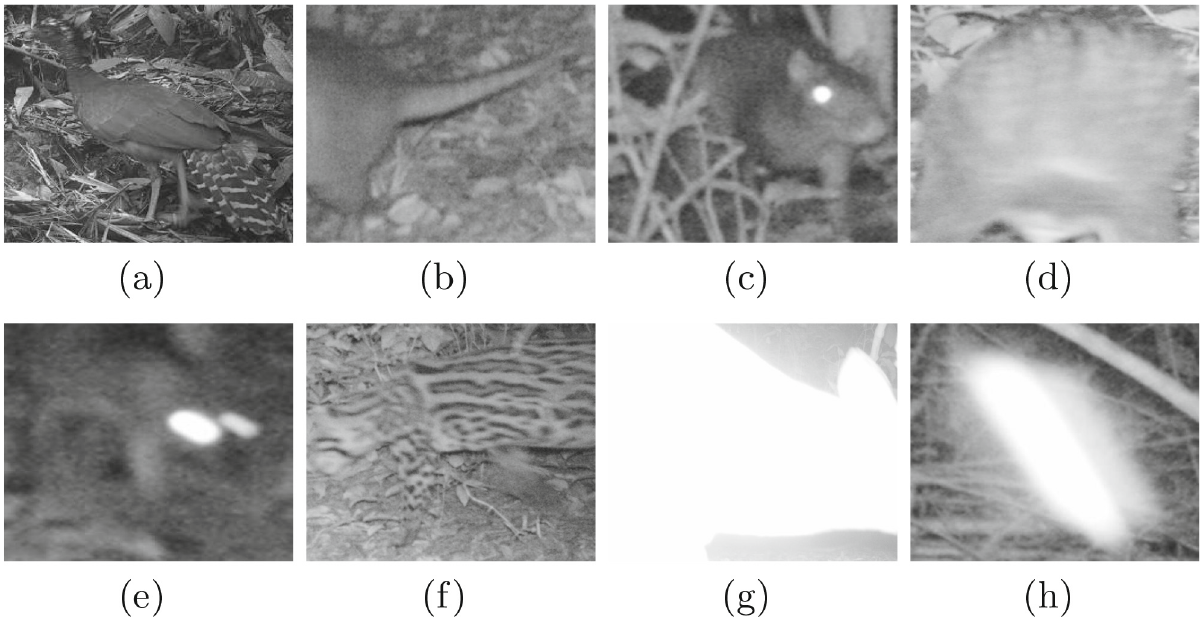
\includegraphics[width=.48\textwidth]{quality}
		\caption{(a) Ideal and scarce case in camera-trap framework. (b) Partial capture of
			the animal. (c) Background occlusion. (d) Auto-occlusion. (e) Low resolution images.
			(f) Blurred animal. (g) Overexposed animal (h) Occlusion of the camera lens.\cite{Gomez:2016:Low}}
		\label{fig:quality}
	\end{figure}

	In order to achieve better results one suggestion from Weinstein \cite{Weinstein:2017} is using image metadata, such as time or location, to assist in image	classification.
	
	For individuals identification, computer vision algorithms use images of known individuals to match new images based on the similarity of phenotypic patterns. 
	By matching the image features among images, matching algorithms score the likelihood that two images are of the same individual. 
	For animals with unique markings, this can be a low-­cost alternative to expensive trapping and tagging programs.
	Current state-of-the-art systems try to solve this problem with highly adapted solutions, which are most of the time not applicable for other areas/species.
	One example of such system is Burghardt's \cite{Burghardt:2016} approach for identifying Great White Sharks individuals based on their fins. 
	It detects and groups object boundaries at multiple scales into an ultrametric contour map.
	Afterwards, salient boundary locations are detected and used to partition region boundaries into contour sections, which  are classified into fin and background classes based on shape, encoded by normals, and local appearance encoded by opponentSIFT features. 
	Other application areas are quite limited, it might be possible to transfer this system to other fish or similar marine creates, for instance dolphins. 
	
	\section{Species Identification}
	
	One of the first approaches for classifying species, which can be seen as similar to identifying individuals, was from Yu \cite{Yu:2013}.
	They reached 82\% accuracy on their dataset of 7196 images and 18 classes with local and global feature extraction, which were used to train an Support Vector Machine (SVM).
	However, this solution still requires a lot of manual preprocessing:
	Removing images without animals, manually cropping all the animals from the images, and selecting only those images that captures the animals' whole body.
	
	The first completely automated approach, which used Deep Learning for species classification was established by Chen \cite{Chen:2014}. 
	They showed that CNNs are able to outperform the traditional Bag-of-Words technique, if enough data is provided. 
	Before training the network, they used their own automatic segmentation method (Ensemble Video Object Cut) for cropping  animals from the images.
	However, the accuracy, which was achieved on their 20,000 image data set with 20 classes, was only 38\%. 
	This can probably be backtracked to their relatively small network architecture, seen in \autoref{fig:chen}
	
	\begin{figure}[htbp]
		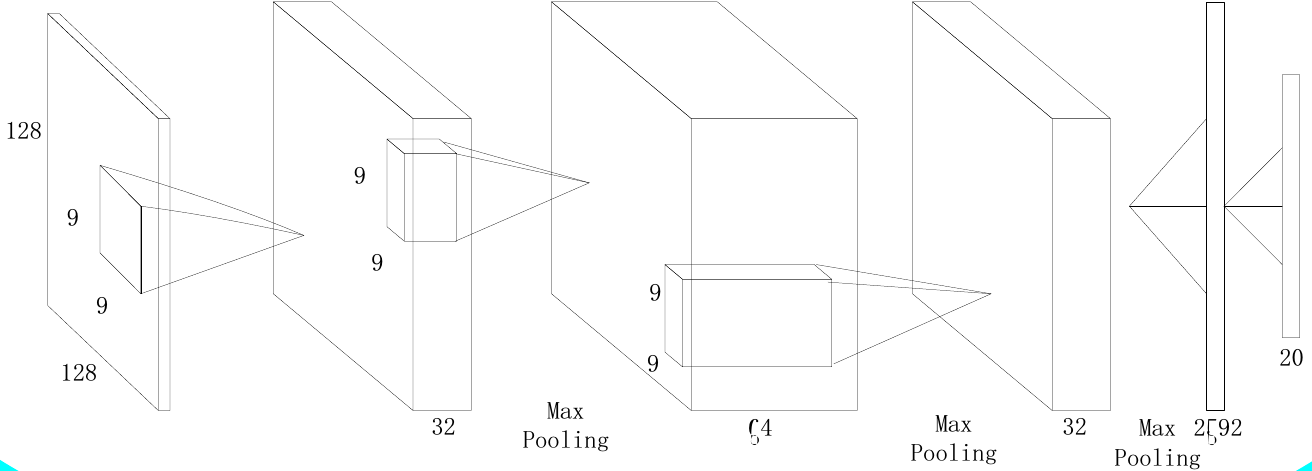
\includegraphics[width=0.48\textwidth]{Chen}
		\caption{The structure of Chen's CNN used for species recognition.\cite{Chen:2014}}
		\label{fig:chen}
	\end{figure}
	
	The work of G\'omez \cite{Gomez:2016:Low} is based on the idea of clustering species to smart biologically inspired sets in order to increase the performance even for low quality as well as gray scale images.
	The data set of 1572 and 2597 images contains animals in the South American jungle, which present a very cluttered back	ground, poor illumination conditions, gray scale, and low resolution.
	In order to increase the trust in the system (necessary due to possible actions e.g. to save species), for each classification a confidence was computed.
	This confidence had to be above a certain threshold or otherwise the images were given to an expert.
	The	training set in the experiments was augmented using images from the ImageNet dataset.
	With regards towards their architecture they utilized several state-of-the-art CNN architectures (AlexNet, VGGNet, GoogLenet and ResNet).
	As preprocessing the images where resized in order to fit the input sizes.
	As a result, they found deeper architectures work better up to ResNet-101, which was found to be the best option for the given dataset. 
	
	A similar approach is from \cite{Gomez:2016}, which uses the Snapshot Serengeti dataset. 
	However, they removed 22 classes that have the fewest images.
	Further, they split up the dataset in order to get unbalanced (rare animals less frequent), balanced (cleaned to get approx. even distribution), conditioned (animals in foreground), and segmented (manually segmented, to simulate perfect segmentation algorithm, which finds (part of) the animal) datasets, which were used during their analysis.
	The used dataset contains high as well as low quality images such as in \autoref{fig:quality2}. 
		
	\begin{figure}[h]
		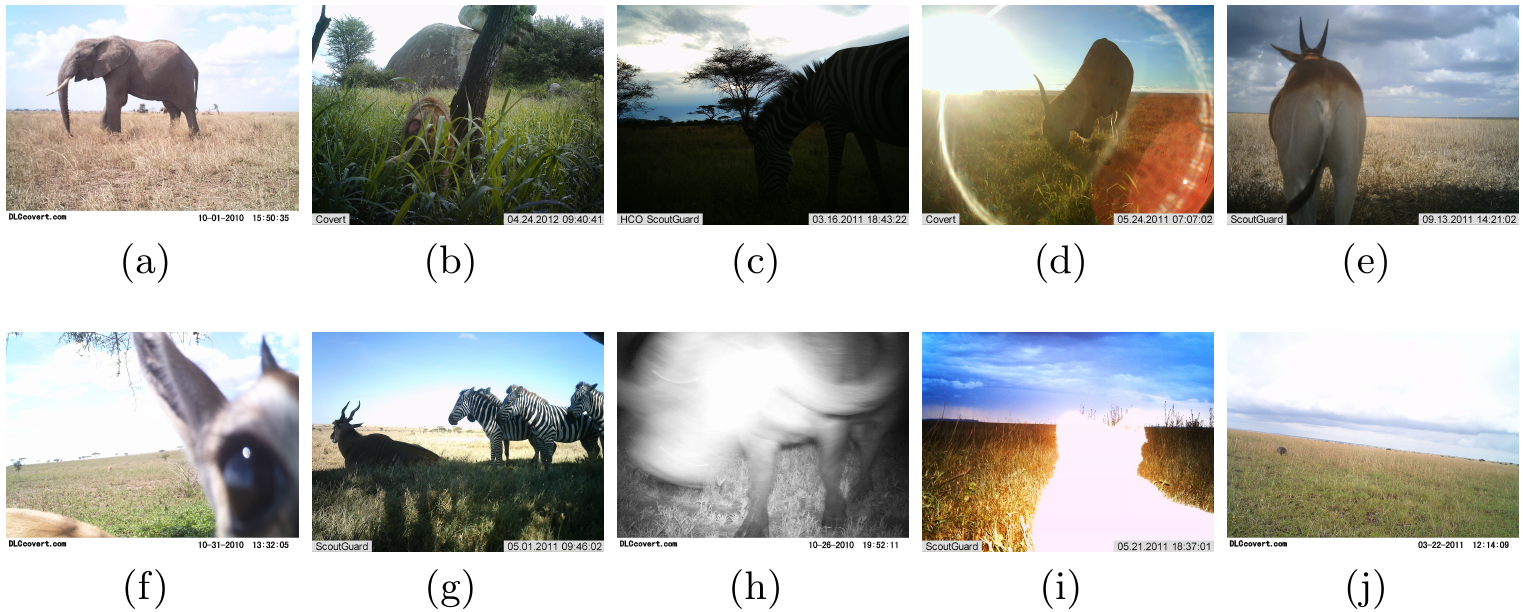
\includegraphics[width=0.48\textwidth]{quality2}
		\caption{ (a) Ideal. (b) Occlusion due
			to context. (c) Poor illumination. (d) Over-exposed regions. (e) Auto-occlusion. (f)	Complex animal poses and unexpected images. (g) Different species in the same image.	(h) Blurred. (i) Over-exposed animals. (j) Animals far way from camera.\cite{Gomez:2016}}
		\label{fig:quality2}
	\end{figure}
	
	They also compared several state-of-the-art CNN architectures (AlexNet, VGGNet, GoogLenet and ResNet).
	The CNNs were all pre-trained with ImageNet and fine-tuned with Stochastic Gradient Descent (SGD) and back-propagation. The Learning rate and step size were reduced to avoid overfitting.
	They found even the deepest architectures cannot deal with highly unbalanced data, but they still perform better than shallow networks.
	For balanced datasets the accuracy increases to 70\%.
	the main problems are empty frames or high distance between camera and animal.
	The conditioned data increased accuracy by 12.9\%, the segmented dataset, however, increased the conditioned result only slightly.
	The suggestion of the paper is to use deeper networks and skip segmentation as well as use sufficiently large datasets.
	
	Another approach based in the Snapshot Serengeti dataset can be found from \cite{Norouzzadeh:2017, Norouzzadeh:2017:Count}. 
	Their research goal was to identify and count species in the Snapshot Serengeti dataset including all 3.2 million images with 48 species. 
	Additionally, they removed images with multiple labels/multiple animals and trained two CNNs for different tasks:
	\begin{itemize}
		\item animal vs. empty (due to 75\% empty frames)
		\item animal identification (species)
	\end{itemize}
	
	Preprocessing includes rescaling the images and normalizing all three input channels individually (z-transformation).
	The training is conducted by using SGD with momentum (0.9), weight decay and batch size of 128.
	The best result was achieved by using VGGNet.
	Nonetheless, ResNet architectures show similar performance with decreases less than 1\% in accuracy.
	In their results they also provide a comparison between pre-trained CNNs as they were used by \cite{Gomez:2016} and CNNs trained from scratch.
	The results suggest that the features learned from the ImageNet dataset do not provide an advantage for learning animal classifications.
	They propose to use pre-trained models on more similar tasks/inputs, so that Deep Learning can also be applied for data sets containing less images than Snapshot Serengeti. 
	Further, their findings show ensembles increase the overall accuracy. 
	One issue with this approach is the low accuracy for rare classes.
	The paper uses weighted loss, oversampling and emphasis sampling to overcome these problems. 
	However, only some classes show improved results with all three methods.
	
	\section{Fine-Grained Object Recognition}
	
	All the above approaches try to solve a fine-grained problem with species identification. 
	Even though some species are really similar, this is definitely true for individuals of the same species.
	
	One approach for fine-grained animal identification can be found from Freytag et al. \cite{Freytag:2014}. 
	Their goal is to identify identity, age, age group, and gender of chimpanzee faces in the wild without the necessity of aligned face images. 
	As mentioned in \autoref{sec:problems} this is often done by highly specific hand-crafted recognition pipelines, which are prone to noise.
	In their experiments they utilize the bilinear pooling approach from \cite{Lin:2015}.
	Further they use matrix logarithm on top of the CNN bilinear pooling ($LOGM$-transformation).
	This transformation can be seen as amplifying axes with small variances in data.
	Intuitively, this is ideal for identification tasks, where small parts of the image are supposed to be discriminative. 
	However, the paper also suggests that for low-quality images bad representations are thereby amplified as well.
	The overall approach was to extract features, which were found in CNNs, apply bilinear pooling and optionally $LOGM$-transformation and finally pass them to a linear SVM after L2-normalizing it.
	Training was done by SGD with weight decay (0.0005), momentum (0.9) and learning rate 0.001 to 0.0001.
	Regarding preprocessing, they found that random crops of 227 px $\times$ 227 px
	after scaling training images to 256 px $\times$ 256 px performed worse than directly scaling images to 227 px $\times$ 227 px.
	The experiments support that bilinear pooling and $LOGM$-transformation show worse results on data with more noise.
	Additionally, they found that pre-trained models on human faces \cite{Parkhi:2015} show much worse results than models trained from scratch. 
	Which is similar to \cite{Norouzzadeh:2017, Norouzzadeh:2017:Count}, where pre-training on ImageNet decreased the performance. 
	Further, feature extraction before the first fully connected layer showed improved results compared to after.
	
	A paper published based on fine-grained recognition is from Branson \cite{Branson:2014}.
	It is working with bird species classification on a dataset containing 11,788 images of 200 bird species.
	The goal was to utilize pose normalization based on aligning detected keypoints to the corresponding keypoints in a prototype image.
	Therefore, they used annotated data, which included parts (namely: image, bounding box, body, head) and keypoints in order to learn how the pictures have to be warped (see \autoref{fig:branson}).
	Based on that they learn the constellation of parts via the deformable part model (DPM) and normalize the parts accordingly.
	
	\begin{figure}[h]
		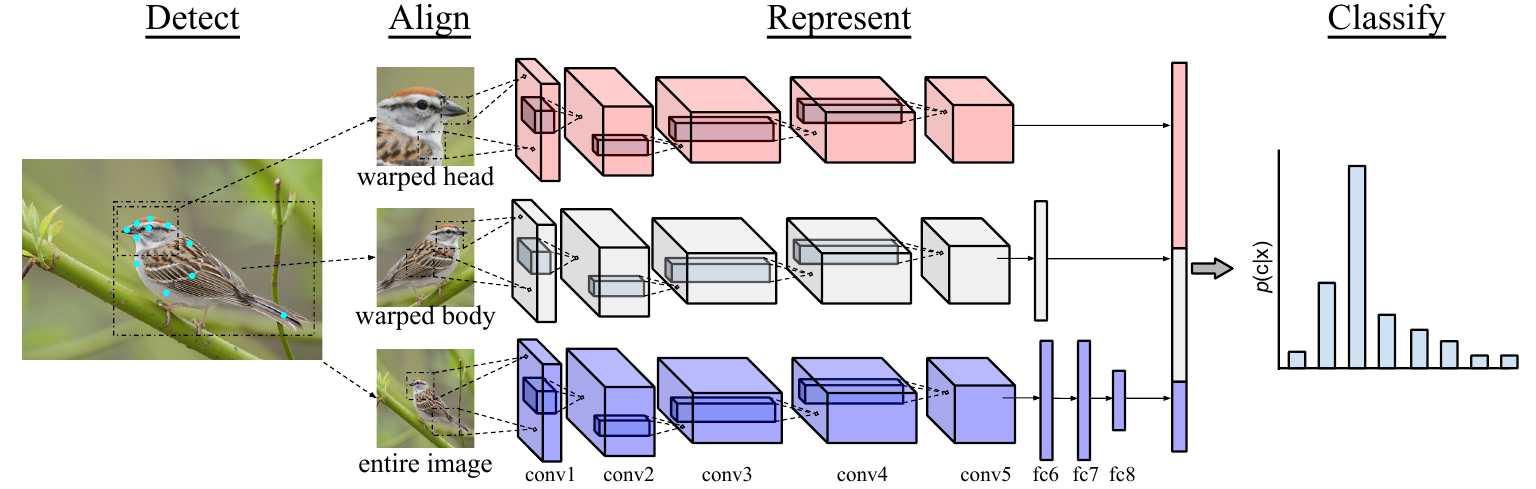
\includegraphics[width=.48\textwidth]{branson-pipeline}
		\caption{Branson's pipeline overview \cite{Branson:2014}}
		\label{fig:branson}
	\end{figure}
	
	They also evaluated a pre-trained model on ImageNet and a fine-tuned version of the same.
	Additionally, they used a third approach, which fine-tuned only the fully connected layer and fixed the other weights.
	The newly learned weights were then used for initialization during the training/fine-tuning of the whole network. 
	In general they saw significant improvements due to the use of CNN features compared to handcrafted models. 
	However, their model drops in performance if no ground truth parts are given and detected parts are used.
	This means, manual annotation of parts is required, which is expensive and often not feasible.
	Further, they found pre-training with ImageNet to be essential in order to achieve good results, which is in contradiction to \cite{Freytag:2014,Norouzzadeh:2017,Norouzzadeh:2017:Count}
	Comparing both fine-tuning methods, the second approach worked more reliable in multiple trails.
	
	The above mentioned bilinear pooling approach from Lin \cite{Lin:2015} focuses more generally on fine-grained recognition. 
	Among others the same bird data set as in \cite{Branson:2014} was used.
	They describe an approach, which has two feature extractors based on CNNs whose outputs are multiplied using the outer product at each location of the image and are pooled across locations to obtain an image descriptor (see \autoref{fig:bilinear}]).
	Their experiments are also different from \cite{Branson:2014} as they do not assume annotated parts or bounding boxes.
	
	\begin{figure}[h]
		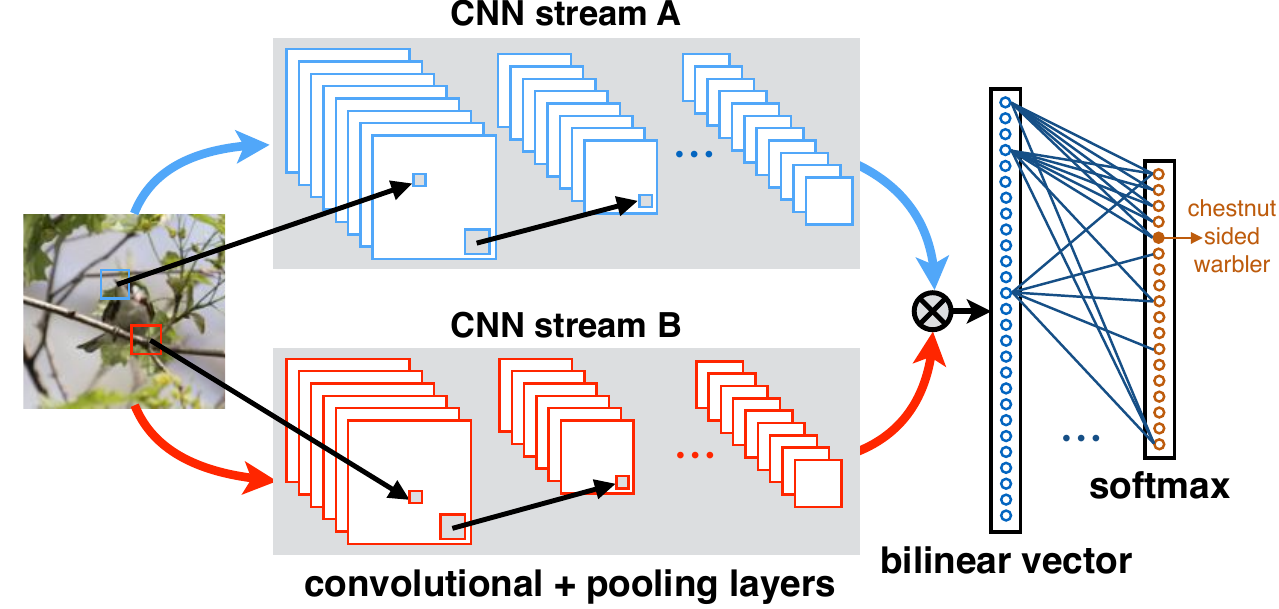
\includegraphics[width=.48\textwidth]{bilinear}
		\caption{A bilinear CNN model for image classification. At	test time an image is passed through two CNNs, A and B, and their outputs are multiplied using outer product at each location of the image and pooled to obtain the bilinear vector. This is passed through a classification layer to obtain predictions.\cite{Lin:2015}}
		\label{fig:bilinear}
	\end{figure}
	
	For their three experiments they used two VGG-M-Nets, two VGG-D-Nets and a combination with one of each. 
	The CNNs are all pre-trained on ImageNet and use only the convolutional layers, which were then combined with bilinear pooling and afterwards l2-normalized.
	For classification they used logistic regression or	linear SVM, which can be replaced by a multi-layer neural network for non-linear outputs.
	Further, they compare the results for input data with annotated bounding boxes and without bounding boxes. 
	Both results where equally good with 84.1\% accuracy and 85.1\% respectively for the combination of VGG-M-Net and VGG-D-Net. 
	In addition, the two VGG-D-Nets performed equally well.
	Problems, which could be found, were the bilinear CNN models that are symmetrically initialized will remain symmetric after fine-tuning. 
	Therefore, they suggest to include Dropout or dimensionality reduction with Principal Component Analysis (PCA) at the end of one CNN.
	With these changes the performance did not increase.
	
	This bilinear pooling model was refined in a later paper from Lin \cite{Lin:2017:Improv}. 
	As found in the above approach, normalization is key to reliable training and prediction. 
	Therefore, they compare different methods of normalization after the bilinear pooling. 
	They propose matrix logarithm and power normalization as possible alternatives (see \autoref{fig:improv-bilinear}.
	
	\begin{figure}[h]
		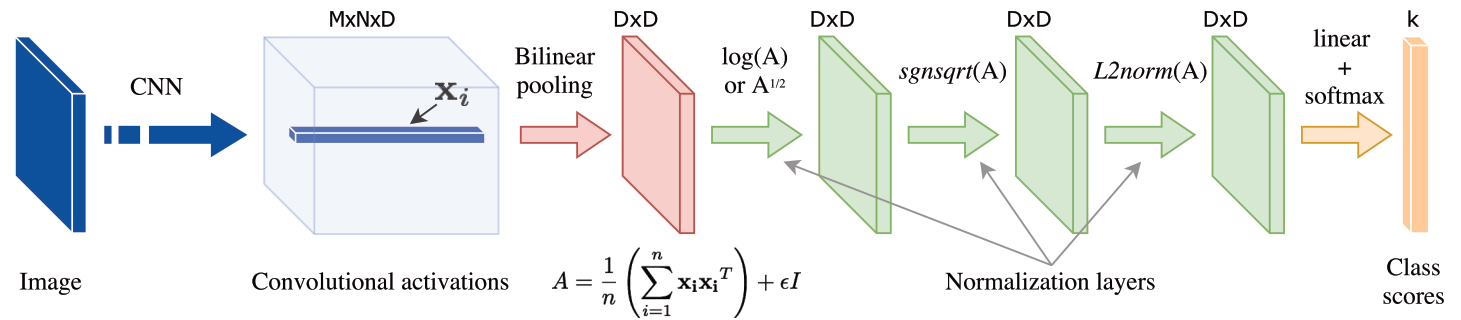
\includegraphics[width=.48\textwidth]{improv-bilinear}
		\caption{Improved B-CNN architecture with a log(A) or A$^\frac{1}{2}$, signed square-root, and l2 normalization layers added after the bilinear pooling of CNN activations.\cite{Lin:2017:Improv}}
		\label{fig:improv-bilinear}
	\end{figure}

	A big drawback they discovered is based on the computation of these normalizations, they normally require Singular Value Decomposition (SVD).
	SVD can be computed during the forward and backward pass, but is highly inefficient (approx. the same time as remaining network).
	They found approximations, based on Denman-Beavers iterations to solve a Lyapunov equation, are a more efficient and suffice for the classification scenario.

	A similar, but different direction as \cite{Branson:2014} is proposed by Simon \cite{Simon:2015}.
	Their goal is to learn model parts completely unsupervised.
	In order to get part proposal they use pre-trained CNNs with ImageNet.
	Also other data sets are possible as the CNN can be pre-trained on a weakly related object dataset.
	The later layers in that CNN are sensitive to increasingly abstract patterns in the image.
	These patterns can correspond to whole objects or parts of objects, which are used as part proposals.
	Nonetheless, one problem is the output resolution at these layers.
	To solve this problem deep neural activation maps are computed, which are used consecutively in order find the part constellations.
	Therefore, different views of objects, i.e. a selection of part proposals are used.
	Shift vectors denote the offset to the common root location of an object.
	This is then formulated as optimization problem of selected view, the common root, the parts proposals associated with a view and if a part is visible or not (see \autoref{fig:bird-norm}).
	
		\begin{figure}[h]
			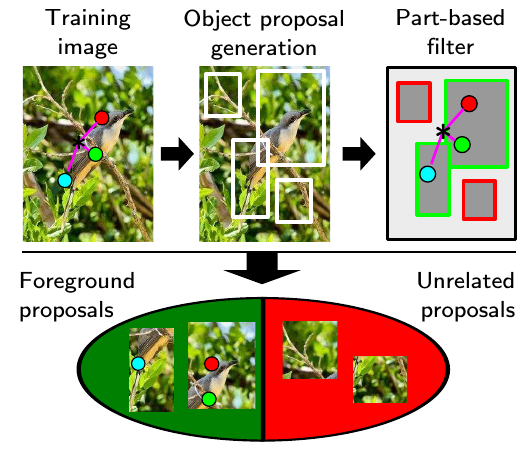
\includegraphics[width=.48\textwidth]{bird-norm}
			\caption{Overview of Simon's approach to filter object proposals for fine-tuning of CNNs\cite{Simon:2015}}
			\label{fig:bird-norm}
		\end{figure}
	
	As result they mainly found improvement, compared to a plain VGGNet without applying part constellations, when classifying the bird datasets.
	On other datasets the performance was similar.
	
	In Gebru's \cite{Gebru:2017} paper a domain adaption approach is proposed. 
	It focuses on learning fine-grained recognition with no or partly labeled data.
	They utilize easily acquirable data, such as data from e-commerce websites, to train the network together with the original data set.
	The goal is to enable fine-grained recognition even for domains where labeling is not economic.
	Further, they try to provide an approach, which avoids training/fine-tuning for every specific topic (e.g. dogs, cats, bunnies, etc.) and instead adapt more general models to real world data.
	For example, images and annotations from a field guide can be used to train a model recognizing various bird species in the wild.
	
	\begin{figure}[h]
		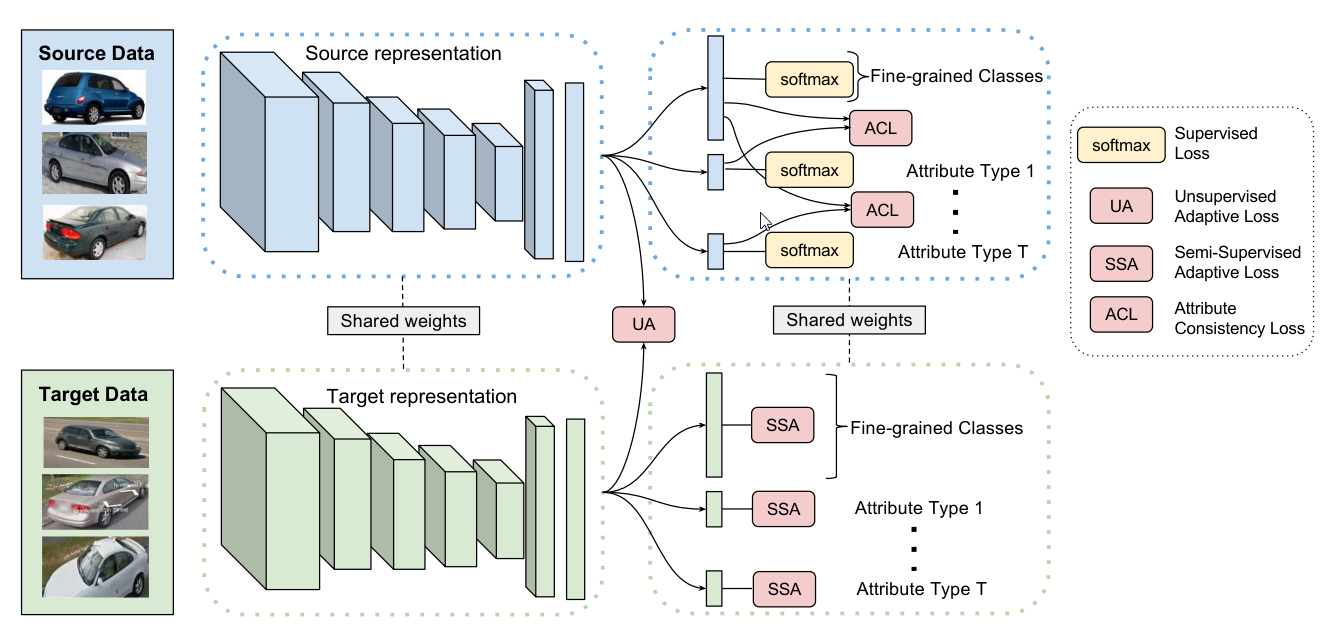
\includegraphics[width=.48\textwidth]{adaption}
		\caption{Architecture overview of Gebru\cite{Gebru:2017}}
		\label{fig:adaption}
	\end{figure}

	As shown in \autoref{fig:adaption}, the idea is based on two CNNs with shared weights.
	One is trained on the easily acquirable source data and the other on the rare target data. 
	They also utilize several independent softmax classification layers in order to predict the fine-grained classes for source and target.
	As mentioned, obtaining labels for every single class is infeasible, however, classes often share attributes. 
	For instance, a Beagle and a Jack Russell terrier are both small dogs while a Bearded Collie and Afghan Hound are both shaggy dogs.
	These attributes are used to in order to identify a target's class more easily.
	During the learning they also included KL Divergence in order to ensure attributes and class predictions are consistent. 
	In their pre-tests, they found that models trained on the source are infeasible for the target data.
	However, a joint training increased the accuracy. 
	In general, the added attributes helped to increase performance further, as long as they are visually informative. 
	For instance, WordNet attributes for an office related data set did not yield in the same results.
	
	\section{Conclusions and Ideas}
	
	Based on the experiments describe previously, a baseline for evaluation needs to be established. 
	A good start for this could be to use a pre-trained VGGNet or ResNet (maybe even use Alex and GooLeNet) in order to predict individuals. 
	In the next steps fine-tuning these models should be tried to validate, which architectures can actually help to solve this problem. 
	If the quality seems to be too low, approaches like Deep image Prior \cite{Ulyanov:2017} could be worth a look.
	Otherwise different crops and flips of the images could improve  training size and generalization.
	In the next stages validating the bilinear pooling model on the dataset is an option.
	Hereby, alternatives of the original implementation could be used, i.e. using different CNN architectures and combining prediction and features extraction in a single network instead of using SVMs afterwards.
	Part detection, part constellation and adaption approaches currently seem quiet complicated to implement using Keras and TF.
	Further, especially the later was published recently and does not provide high accuracy scores.
	First, the above ideas should be evaluated.
	
	
	
	%----------------------------------------------------------------------------------------
	%	BIBLIOGRAPHY
	%----------------------------------------------------------------------------------------
	
	%\bibliographystyle{abbrv}
	\bibliographystyle{abbrv-doi}
	%\bibliographystyle{abbrv-doi-narrow}
	%\bibliographystyle{abbrv-doi-hyperref}
	%\bibliographystyle{abbrv-doi-hyperref-narrow}
	
	\bibliography{sources}
	
	%----------------------------------------------------------------------------------------


\end{document}
